\section*{Question 1}

\begin{custombox}[label={box:Q1}]{Question 1}
	In $E1$ you have already created a dataset $(y, x)$. Calculate the \textbf{Pearson Correlation Coefficient} $(r)$ for this dataset and comment on the value.
\end{custombox}

We calculate the Pearson Correlation Coefficient $(r)$ as follows:

\begin{align}
	r &= \frac{\sum_{i=1}^{n} (x_i - \bar{x})(y_i - \bar{y})}{\sqrt{\sum_{i=1}^{n} (x_i - \bar{x})^2 \sum_{i=1}^{n} (y_i - \bar{y})^2}}
\end{align}

where $\bar{x}$ and $\bar{y}$ are the means of $x$ and $y$ respectively.

% \begin{figure}[H]
% 	\centering
% 	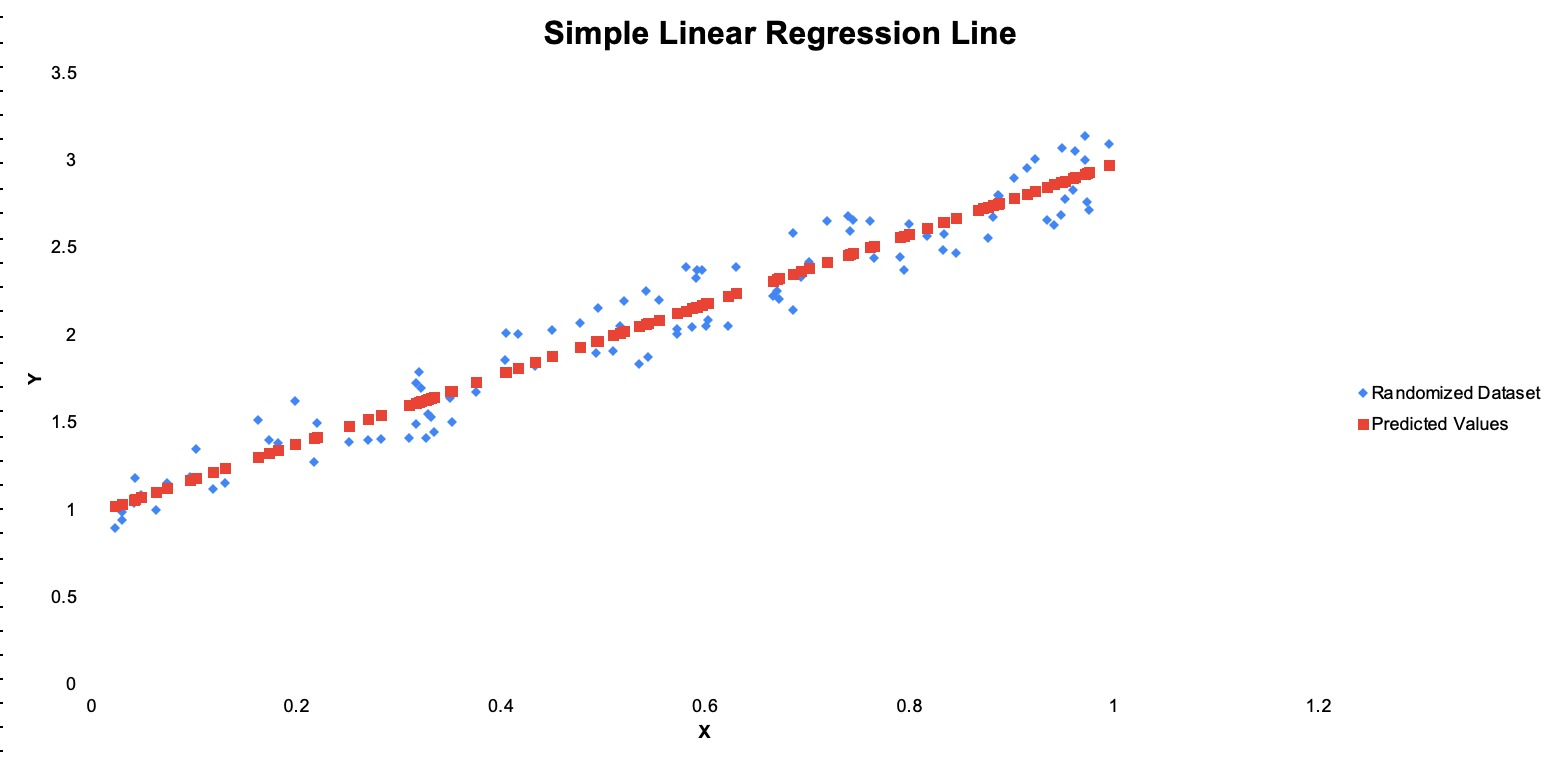
\includegraphics[width=0.8\textwidth]{Images/Q1_2.jpeg}
% 	\caption{Scatter plot of the dataset $(y, x)$ along with the regression line}
% 	\label{fig:Q1_2}
% \end{figure}

\begin{figure}[H]
	\centering
	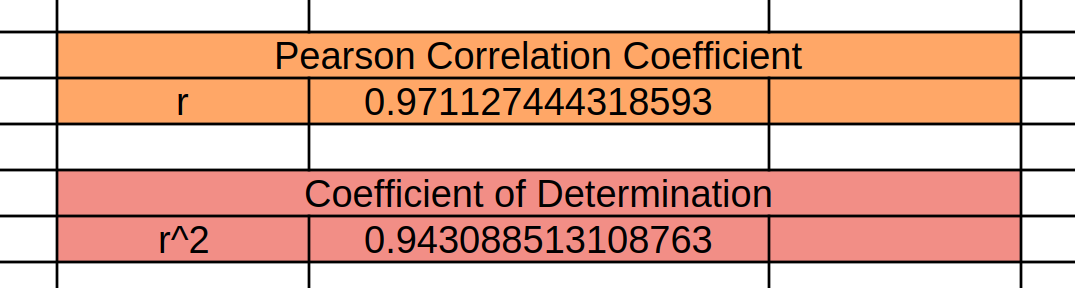
\includegraphics[width=0.4\textwidth]{Images/Q1.png}
	\caption{Pearson Correlation Coefficient $(r)$}
	\label{fig:Q1}
\end{figure}

\clearpage



